\documentclass{beamer}%[hyperref={backref=slide}]

%\input{sl_slide_preamble.tex}
\input{sl_slide_preamble_nonotes.tex}
\input{sl_slide_graphics_preamble.tex}
\input{sl_definitions.tex}
\input{sl_slide_symbols.tex}
%
\graphicspath{{"Figures/"}}
\DeclareMathOperator{\SNR}{SNR}
\DeclareMathOperator{\snr}{SNR}
%matrices
\newcommand{\inv}{^{-1}}
\newcommand{\I}{\mathbf{I}}
%prob vector
\newcommand{\pr}{\mathbf{p}}
%equilibrium distribution
\newcommand{\eq}{\pr^\infty}
%first passage times
\newcommand{\fpt}{\mathbf{T}}
%off-diag first passage times
\newcommand{\fptb}{\overline{\fpt}}
%other symbols
\newcommand{\w}{\mathbf{w}}
\newcommand{\W}{\mathbf{W}}
\newcommand{\frg}{\W^\mathrm{F}}
\newcommand{\M}{\mathbf{M}}
\newcommand{\F}{\boldsymbol{\Phi}}
\newcommand{\wv}{\vec{w}}
%super/subscripts
\newcommand{\pot}{^{\text{pot}}}
\newcommand{\dep}{^{\text{dep}}}
\newcommand{\potdep}{^{\text{pot/dep}}}
\newcommand{\lmax}{_{\text{max}}}
\newcommand{\lmin}{_{\text{min}}}
%quantities
\newcommand{\initial}{\mathcal{I}}
\newcommand{\area}{\mathcal{A}}
\newcommand{\CS}{\mathcal{S}}
\newcommand{\comp}{^\mathrm{c}}
\renewcommand{\e}{\mathsf{e}}
%---------Title-----------------------------------------------------------

\title[Complex synapses]{A general theory of learning and memory with Complex Synapses}
%
%\subtitle{\small{based on ``A memory frontier for complex synapses''.
%\newblock Subhaneil Lahiri and Surya Ganguli.
%\newblock
%  \href{http://papers.nips.cc/paper/4872-a-memory-frontier-for-complex-synapses.pdf}{In
%  C.J.C. Burges, L.~Bottou, M.~Welling, Z.~Ghahramani, and K.Q. Weinberger,
%  editors, \emph{Advances in Neural Information Processing Systems 26}, pages
%  1034--1042. }2013.
%}
%}
%
\author{Subhaneil Lahiri%\inst{1}
}
%
\institute[Stanford]{%
%\inst{1}
Stanford University, Applied Physics
}

%---------Beginning--------------------------------------------------------

\begin{document}

%-------------Slide--------------------------------------------------------

\begin{frame}
%
 \titlepage
 \begin{center}
 \small{see: S.~Lahiri and S.~Ganguli, ``\emph{A memory frontier for complex synapses},''
 \\
  \href{http://papers.nips.cc/paper/4872-a-memory-frontier-for-complex-synapses.pdf}{\emph{Advances in Neural Information Processing Systems 26}, pages
  1034--1042. }2013.
}
\end{center}
%
\end{frame}

%-------------Slide--------------------------------------------------------

\begin{frame}{Synapses are complex}
%
 \parbox[t]{0.45\linewidth}{%
 \includegraphics[height=0.8\linewidth]{2000102CobaFig4.pdf}

 \citerr{Coba2009phosphorylation}
 }
 \hspace{0.05\linewidth}
 \parbox[t]{0.45\linewidth}{%
 \hfill
 \includegraphics[height=0.8\linewidth]{MadisonMontgomery.jpg}

 \citerr{Montgomery2002765}
 }
%
\end{frame}

%-------------Slide--------------------------------------------------------

\begin{frame}{Models of complex synaptic dynamics}
%
%  There are $N$ identical synapses with $M$ internal functional states.
\parbox[c]{0.82\linewidth}{%
  \begin{itemize}
    \item Internal functional state of synapse \lto\ synaptic weight.
    \item Candidate plasticity events \lto\ transitions between states
  \end{itemize}
}\hfill
\alignmid{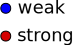
\includegraphics[width=0.13\linewidth]{state_key.svg}}
  %
  \vp
  \begin{center}
%  \begin{overlayarea}{0.7\linewidth}{0.3\linewidth}
%    \only<1>{\includegraphics[width=0.99\linewidth]{synapse_model_1.svg}}%
%    \only<2>{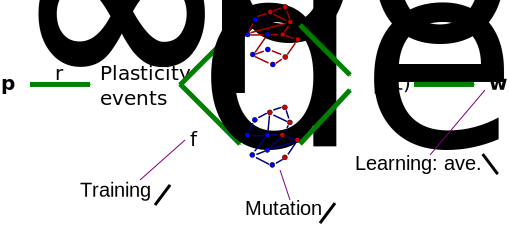
\includegraphics[width=0.99\linewidth]{synapse_model_2.svg}}
%  \end{overlayarea}
%    \aligntop{\movie[width=200px,height=92px,showcontrols=true,loop]{\includegraphics[width=200px,height=92px]{Vids/plast_00.png}}{plast.avi}}
    \only<1>{\aligntop{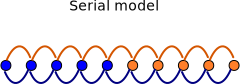
\includegraphics[width=0.5\linewidth]{Animation/serial.svg}}}%
    \only<2>{\aligntop{\includegraphics[width=0.5\linewidth]{Animation/serial_anim_01.svg}}}%
    \only<3>{\aligntop{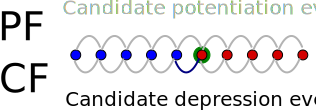
\includegraphics[width=0.5\linewidth]{Animation/serial_anim_02.svg}}}%
    \only<4>{\aligntop{\includegraphics[width=0.5\linewidth]{Animation/serial_anim_03.svg}}}%
%    \only<5>{\aligntop{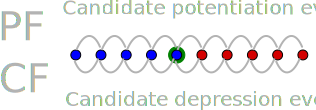
\includegraphics[width=0.5\linewidth]{Animation/serial_anim_04.svg}}}%
%    \only<6>{\aligntop{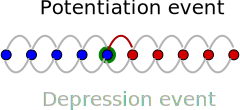
\includegraphics[width=0.5\linewidth]{Animation/serial_anim_05.svg}}}%
%    \only<7>{\aligntop{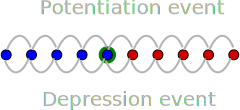
\includegraphics[width=0.5\linewidth]{Animation/serial_anim_06.svg}}}%
%    \only<8>{\aligntop{\includegraphics[width=0.5\linewidth]{Animation/serial_anim_07.svg}}}%
%    \only<9>{\aligntop{\includegraphics[width=0.5\linewidth]{Animation/serial_anim_08.svg}}}%
%    \only<10>{\aligntop{\includegraphics[width=0.5\linewidth]{Animation/serial_anim_09.svg}}}%
%    \only<11>{\aligntop{\includegraphics[width=0.5\linewidth]{Animation/serial_anim_10.svg}}}%
%    \only<12>{\aligntop{\includegraphics[width=0.5\linewidth]{Animation/serial_anim_11.svg}}}%
%    \only<13>{\aligntop{\includegraphics[width=0.5\linewidth]{Animation/serial_anim_12.svg}}}%
%    \only<14>{\aligntop{\includegraphics[width=0.5\linewidth]{Animation/serial_anim_13.svg}}}%
%    \only<15>{\aligntop{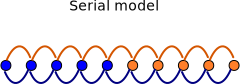
\includegraphics[width=0.5\linewidth]{Animation/serial.svg}}}%
    \only<5>{\aligntop{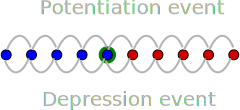
\includegraphics[width=0.5\linewidth]{Animation/serial_anim_06.svg}}}%
    \only<6>{\aligntop{\includegraphics[width=0.5\linewidth]{Animation/serial_anim_07.svg}}}%
    \only<7>{\aligntop{\includegraphics[width=0.5\linewidth]{Animation/serial_anim_08.svg}}}%
    \only<8>{\aligntop{\includegraphics[width=0.5\linewidth]{Animation/serial_anim_09.svg}}}%
    \only<9>{\aligntop{\includegraphics[width=0.5\linewidth]{Animation/serial_anim_10.svg}}}%
    \only<10>{\aligntop{\includegraphics[width=0.5\linewidth]{Animation/serial_anim_11.svg}}}%
    \only<11>{\aligntop{\includegraphics[width=0.5\linewidth]{Animation/serial_anim_12.svg}}}%
    \only<12>{\aligntop{\includegraphics[width=0.5\linewidth]{Animation/serial_anim_13.svg}}}%
    \only<13>{\aligntop{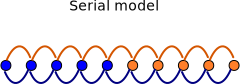
\includegraphics[width=0.5\linewidth]{Animation/serial.svg}}}%
    %
%    \hspace{0.05\linewidth}\parbox[t]{0.45\linewidth}{\raggedright
%    \visible<13>{
%    Mutation: trans.\ probs. \\ \vp
%    Training: rates of pot/dep events \\ \vp
%    Learning: synaptic weight}}
  \end{center}

%  \onslide<2>{\hfill
%  \parbox[t]{0.3\linewidth}{PF+\cancel{CF} \lto\ LTP, \\
%              PF+CF \lto\ LTD.}
%  \parbox[t]{0.27\linewidth}{Lower threshold\\ for LTD}
%  \parbox[t]{0.27\linewidth}{VOR gain increase}}

  \vp
  \footnotesize\citerr{Fusi2005cascade,Fusi2007multistate,Barrett2008discrete}\\\citerr{Lahiri2013synapse}

  %
  \note[item]{complex synapse: not just synaptic weight. dynamical system}
  \note[item]{important for memory with bounded synapses}
  \note[item]{nodes \lto\ states}
  \note[item]{color \lto\ sttrength}
  \note[item]{arrows \lto\ plasticity}
%  \note[item]{stoch process has steady state distribution.}
%  \note[item]{Prior activity puts it in this state. row vec.}
  \note[item]{plasticity events at rate r. indep at each synapse.}
  \note[item]{fraction pot/dep}
  \note[item]{Readout: synaptic weight vec when in each state.}
    \note[item]{Mutation: lower threshold \lto\ increase transition probs}
    \note[item]{Training: Changes statistics of LTP/LTD. Only parameters we have. Don't care about $r$.}
    \note[item]{Learning: Only output we have. Don't keep track of synaptic identity.}
%    \note<2>[item]{Same PF+CF input \lto\ same $r,f\pot,f\dep$ in each case.}
%    \note<2>[item]{Input to Pk, some linear combination of $\w$'s. }
% At $t=0$, the memory is created by $\M\potdep$ with probability $f\potdep$.
% \note[item]{for this one, we keep track of pot/dep, look for inc/dec of $\w$}
%
% \vp Forgetting caused by subsequent memories, evolving as
%
%  \begin{equation*}
%  \begin{aligned}
%    \diff{\pr(t)}{t} &= r\pr(t)\frg,
%    &\qquad
%    \frg &= f\pot\M\pot+f\dep\M\dep-\I,\\&&
%    \eq\frg &=0.
%  \end{aligned}
%  \end{equation*}
%%
%  \note[item]{Memory at $t=0$, keep track of pot/dep}
%  \note[item]{subsequent: average over pot/dep}
% \note[item]{$\frg$ is forgetting matrix, $\I=$identity, don't keep track of pot/dep}
% Eventually, this will settle into the equilibrium distribution:
% %
% %
% \note[item]{In equilibrium prior to memory creation}
%
\end{frame}

%-------------Slide--------------------------------------------------------

\begin{frame}{Example models}
%
 Two example models of complex synapses.
 %
 \begin{center}
  \aligntop{\includegraphics[width=4cm]{cascade.svg}}
  \hspace{2cm}
  \aligntop{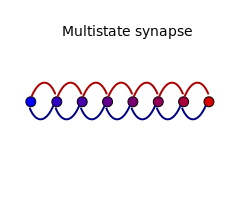
\includegraphics[width=4cm]{multistate.svg}}
 \end{center}
 \citerr{Fusi2005cascade,Leibold2008serial,Ben-DayanRubin2007sparse}
 %
 \note[item]{previous work, also: Benna-Fusi}

 These have different memory storage properties
 %
 \begin{center}
 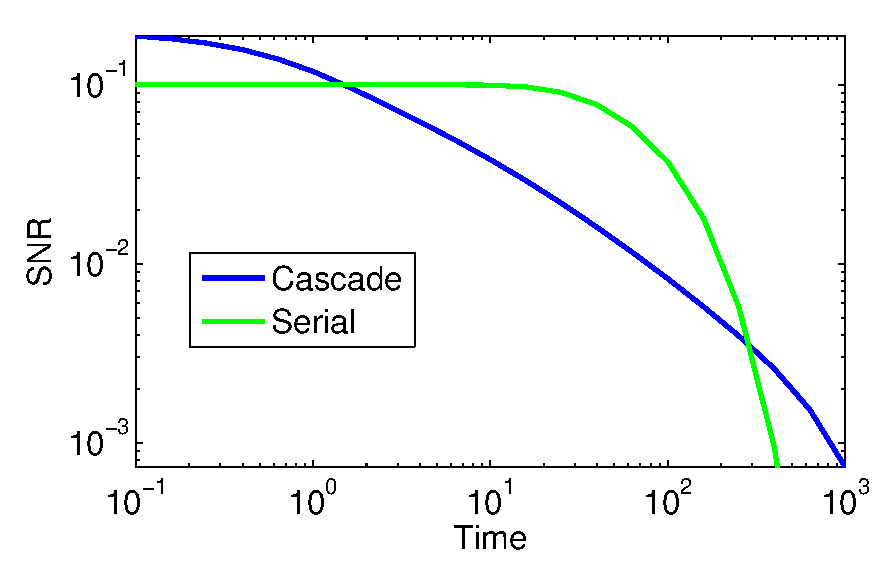
\includegraphics[width=0.5\linewidth]{cascms.eps}
 \end{center}
 %
 \note[item]{Multistate good at one time, bad at others,}
 \note[item]{Cascade, less well at that time, better over range of times.}
%
\end{frame}

%-------------Slide--------------------------------------------------------

\begin{frame}{Memory curve envelope}
%
 %
% \begin{center}
 \parbox[c]{0.58\linewidth}{
   \only<1>{\aligntop{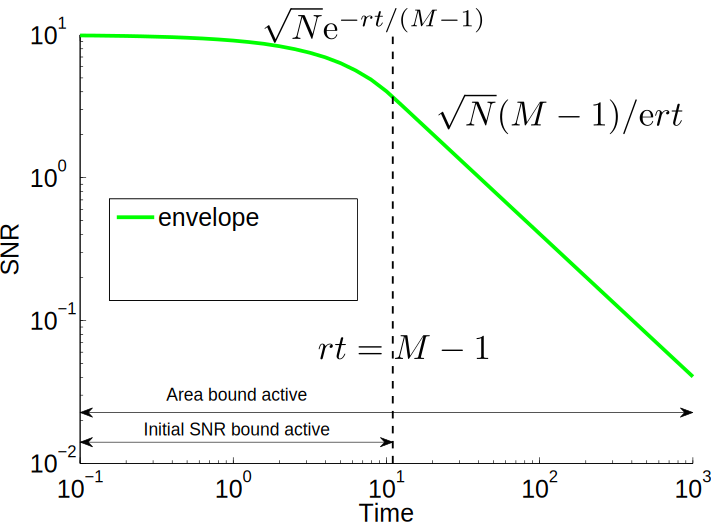
\includegraphics[width=0.95\linewidth]{env_only.svg}}}%
   \only<2>{\aligntop{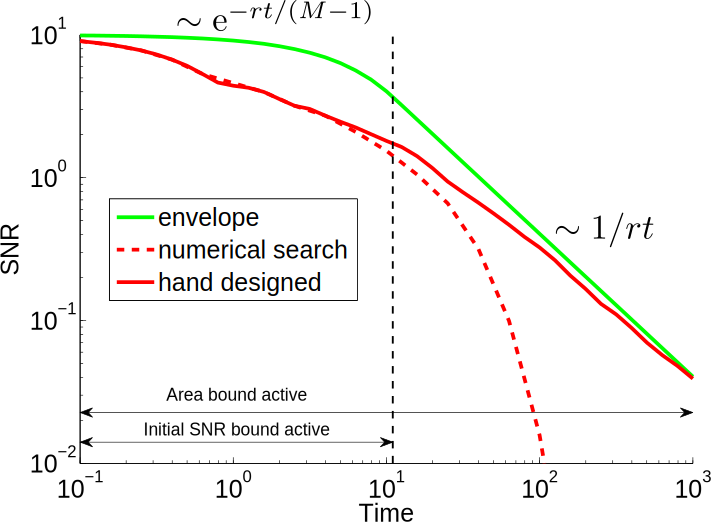
\includegraphics[width=0.95\linewidth]{env.svg}}}
   \note[item]{Best we've found, by numerical opt and hand chosen models.}
% \note[item]{Models on next slide}
 }
% \end{center}
 \hp
 %
 \parbox[c]{0.36\linewidth}{
 \visible<2>{
   Early times (vary \# states):
   %
   \begin{center}
  %   \includegraphics[width=6cm]{multistate_shorten.svg}
     \includegraphics[width=0.99\linewidth]{diffjump.svg}
   \end{center}
   %
  % \note[item]{shorten length of chain, keeping deterministic}
   \note[item]{vary length, keeping deterministic}
   %
   Late times (vary $\varepsilon$.):
   %
   \begin{center}
     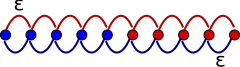
\includegraphics[width=0.99\linewidth]{multistate_sticky.svg}
   \end{center}
   %
   }
   \note[item]{Area maximising.}
 }
 \note[item]{Gap $\sim\CO(\sqrt{N})$.}
 \note[item]{Area bound active at early times $\implies$ need more constraints.}
%
\end{frame}



%-------------Slide--------------------------------------------------------
\appendix

\begin{frame}[allowframebreaks]{References}
%

 {\small
 \bibliographystyle{unsrt_slides}
 \bibliography{maths,neuro}
 }
%
\end{frame}

%-----End----------------------------------------------------------------

\end{document}
